\begin{appendices}
\appendix
\chapter{Study Tasks}

% =========================
% Task Group 1
% =========================
\section[Github Repo Explanation]{COPILOT-VIBE-AGENTIC-CODING-STUDY}
\label{app:repo}
\begin{lstlisting}[language=]
# Copilot Vibe Agentic Coding Study

This repository contains coding tasks for a study comparing two modes of GitHub Copilot: Vibe Coding (Ask Mode) and Agentic Coding (Agent Mode).

## Participant Groups

- **Group 1 (GAIA-inspired Tasks):** Data analysis and CSV processing tasks using Python's standard library.
  - Assigned tasks: `task_group_1/task_1a/` and `task_group_1/task_1b/`.
- **Group 2 (SWE-inspired Tasks):** Bug-fixing tasks in Python configuration parsers.
  - Assigned tasks: `task_group_2/task_2a/` and `task_group_2/task_2b/`.

You will be assigned to one group based on the study design.

## Repository Contents

- `task_group_1/`: Data Analysis Tasks (Group 1)
  - `task_1a/`: **GAIA-a - Invasive Species Research**: Analyze USGS CSV data to find unique ZIP codes where clownfish (from *Finding Nemo*) was observed as nonnative before 2020. Filter by species name, data source, and observation year. Return sorted list of 5-digit ZIP codes.
  - `task_1b/`: **GAIA-b - British Museum Mollusk Shell & Bead Age**: Analyze research articles CSV to find the minimum age of beads made from a specific mollusk species linked to British Museum object "2012,5015.17". Filter by journal (Science Advances), publication year (2021), and return minimum age in thousands of years.

- `task_group_2/`: Software Engineering Bug-Fixing Tasks (Group 2)
  - `task_2a/`: **CSV Parser Case Sensitivity Bug**: Fix a CSV configuration parser that crashes on lowercase commands. The parser reads special command lines (like `#SKIP` or `#DELIMITER`) but only recognizes UPPERCASE versions. Make command parsing case-insensitive so `#skip`, `#Skip`, and `#SKIP` all work.
  - `task_2b/`: **JSON Config Validation Bug**: Fix a configuration validator that fails to handle boolean values represented as strings. Add support for converting string representations (`"true"`, `"false"`, `"1"`, `"0"`) to proper boolean types, similar to existing int/float conversion.

- Each task folder has its own README with detailed instructions, starter code, tests, and data files (for Group 1).

## Experiment Process (Step-by-Step)

The study takes 60 minutes total. Follow these steps in order:

1. **Phase 1: Onboarding & Consent (10 minutes)**
   - Arrive and review the study procedure.
   - Sign consent form.
   - Complete a background survey (experience with AI tools, programming).

2. **Phase 2: Task 1 Coding Session (15 minutes)**
   - The researcher assigns you a Copilot mode (Vibe or Agentic) for this task.
   - Navigate to your assigned task folder (based on your group).
   - Read the task README and implement the code using the assigned mode.
   - Screen recording and time tracking will occur.

3. **Phase 3: Post-Task Survey 1 (5 minutes)**
   - Complete a short survey rating the mode you just used.
   - Sample questions (Likert scale: 1-5, Strongly Disagree to Strongly Agree):
     - "I trusted the AI suggestions."
     - "The mode aligned with my workflow."
     - "I felt in control of the coding process."
   - Write a brief reflection (e.g., "What was frustrating?").

4. **Phase 4: Task 2 Coding Session (15 minutes)**
   - Switch to the other Copilot mode.
   - Work on the second task in your group.
   - Screen recording continues.

5. **Phase 5: Post-Task Survey 2 (5 minutes)**
   - Rate the second mode with similar Likert questions.
   - Write a brief reflection.

6. **Phase 6: Comparative Interview (10 minutes)**
   - Discuss your experiences with both modes.
   - Answer comparative questions (e.g., "Which mode was more efficient?").

**Important:** Stick to the time limits. Do not switch modes mid-task. The researcher will guide you through each phase.

\end{lstlisting}
\section{Task Group 1}
Task materials are provided in Appendix~\ref{app:tg1a-code} and Appendix~\ref{app:tg1b-code}.

\begin{figure}[ht]
\setlength{\fboxsep}{5pt}
\centering
\begin{minipage}[t]{1\textwidth}
\fbox{%
\parbox{\textwidth}{\footnotesize
\textbf{Task Group 1 (TG1): Data analysis tasks}\par\medskip
\texttt{task\_group\_1/}\\
\texttt{├─ task\_1a/}\\
\texttt{│\ \ ├─ README.md}\\
\texttt{│\ \ ├─ data/ \ \ \ \ \ (CSV)}\\
\texttt{│\ \ ├─ src/ \ \ \ \ \ (solution.py)}\\
\texttt{│\ \ └─ tests/ \ \ (test\_solution.py)}\\
\texttt{└─ task\_1b/}\\
\texttt{\hspace*{1.6em}├─ README.md}\\
\texttt{\hspace*{1.6em}├─ data/ \ \ \ \ \ (CSV)}\\
\texttt{\hspace*{1.6em}├─ src/ \ \ \ \ \ (solution.py)}\\
\texttt{\hspace*{1.6em}└─ tests/ \ \ (test\_solution.py)}\\
}}
\end{minipage}
\end{figure}

\subsection{Task 1a}
\label{app:tg1a-code}
\begin{lstlisting}[language=]
# task_group_1/task_1a/README.md
# Task Group 1: Data Analysis Tasks

## Steps to Complete Task Group 1

1. Install Python
   - Download and install Python 3.6+ from [python.org](https://www.python.org/downloads/)
   - Verify installation: `python --version`
   - Ensure pip is available: `pip --version`
     - If not, install via `python get-pip.py` (download from bootstrap.pypa.io) or `python -m ensurepip --upgrade`

2. Set up the project environment
   - Navigate to the task directory: `cd task_group_1/task_1a/`
   - (Optional) Create a virtual environment for isolation: `python -m venv venv` then activate it
   - Install testing dependencies: `python -m pip install pytest` (use `python -m pip` instead of `pip` directly, as `pip` may not be in PATH)
   - *Note for macOS/Apple users: If you encounter issues, you may need to install Python via Homebrew (`brew install python3`) or use `python3` instead of `python`*

3. Implement the solution
   - Read `task_1a/README.md` for details
   - Edit `task_1a/src/solution.py` to implement the required function

4. Run and validate the solution
   - Execute tests: `python -m pytest` (from `task_1a/` directory)
   - Ensure all tests pass

# GAIA-a – Invasive Species Research (Data Analysis Task)

## Task Overview

Analyze a CSV of USGS invasive species records for a pet fish from *Finding Nemo*. Find all unique 5-digit ZIP codes where this fish was observed as nonnative before 2020. Do not use web access or external APIs.

## Files and Structure

```
.
├─ README.md                # This file
├─ data/
│  └─ usgs_nemo_observations.csv
├─ src/
│  └─ solution.py           # Implement your solution here
└─ tests/
   └─ test_solution.py      # Automated tests
```

### data/usgs_nemo_observations.csv

CSV with columns: `species_common_name`, `data_source`, `observation_year`, `zip_code`, etc. Inspect header for exact names.

## What You Need to Implement

Implement in `src/solution.py`:

```python
from typing import List

def find_nonnative_zip_codes(csv_path: str = "data/usgs_nemo_observations.csv") -> List[str]:
    """
    Return unique 5-digit ZIP codes where the Nemo fish (clownfish) was observed as nonnative by USGS before 2020.
    Filter: data_source == "USGS", observation_year < 2020, species contains "clownfish" (case-insensitive).
    Return sorted list of strings.
    """
    ...
```

## Input / Output

- **Input:** CSV path (default: "data/usgs_nemo_observations.csv")
- **Output:** List[str] of unique ZIP codes, sorted ascending.

Example: ["33040", "60601", "96701", "96706", "96734"]

## Constraints

- Python 3, standard library only.
- Do not modify CSV or test files.

## Evaluation

Tests check correct filtering, unique/sorted ZIP codes, and match expected results.

## Hints

- Use `csv` module.
- Lowercase for species matching.
- ZIP codes as strings to preserve leading zeros.
- Use `set` for uniqueness, then sort.

---

# Görev Grubu 1: Veri Analizi Görevleri

## Görev Grubu 1'i Tamamlama Adımları

1. Python'u Yükleyin
   - Python 3.6+ sürümünü [python.org](https://www.python.org/downloads/) adresinden indirip yükleyin
   - Kurulumu doğrulayın: `python --version`
   - pip'in mevcut olduğundan emin olun: `pip --version`
     - Değilse, `python get-pip.py` (bootstrap.pypa.io'dan indirin) veya `python -m ensurepip --upgrade` ile yükleyin

2. Proje ortamını kurun
   - Görev dizinine gidin: `cd task_group_1/task_1a/`
   - (İsteğe bağlı) İzolasyon için sanal ortam oluşturun: `python -m venv venv` ardından aktif edin
   - Test bağımlılıklarını yükleyin: `python -m pip install pytest` (PATH'te olmayabileceğinden `pip` yerine `python -m pip` kullanın)

3. Çözümü uygulayın
   - Detaylar için `task_1a/README.md` dosyasını okuyun
   - Gerekli fonksiyonu uygulamak için `task_1a/src/solution.py` dosyasını düzenleyin

4. Çözümü çalıştırın ve doğrulayın
   - Testleri çalıştırın: `python -m pytest` (`task_1a/` dizininden)
   - Tüm testlerin geçtiğinden emin olun

# GAIA-a – İstilacı Tür Araştırması (Veri Analizi Görevi)

## Görev Özeti

*Finding Nemo* filminden bir evcil balık için USGS istilacı tür kayıtlarının bulunduğu bir CSV dosyasını analiz edin. Bu balığın 2020'den önce yerli olmayan tür olarak gözlemlendiği tüm benzersiz 5 haneli posta kodlarını bulun. Web erişimi veya harici API kullanmayın.

## Dosyalar ve Yapı

```
.
├─ README.md                # Bu dosya
├─ data/
│  └─ usgs_nemo_observations.csv
├─ src/
│  └─ solution.py           # Çözümünüzü buraya uygulayın
└─ tests/
   └─ test_solution.py      # Otomatik testler
```

### data/usgs_nemo_observations.csv

Sütunları içeren CSV: `species_common_name`, `data_source`, `observation_year`, `zip_code`, vb. Tam isimler için başlığı inceleyin.

## Uygulamanız Gerekenler

`src/solution.py` dosyasında uygulayın:

```python
from typing import List

def find_nonnative_zip_codes(csv_path: str = "data/usgs_nemo_observations.csv") -> List[str]:
    """
    Nemo balığının (palyaço balığı) 2020'den önce USGS tarafından yerli olmayan tür olarak 
    gözlemlendiği benzersiz 5 haneli posta kodlarını döndürün.
    Filtre: data_source == "USGS", observation_year < 2020, tür adında "clownfish" içerir (büyük/küçük harf duyarsız).
    Sıralanmış string listesi döndürün.
    """
    ...
```

## Girdi / Çıktı

- **Girdi:** CSV dosya yolu (varsayılan: "data/usgs_nemo_observations.csv")
- **Çıktı:** Artan sırada sıralanmış benzersiz posta kodlarının List[str] listesi.

Örnek: ["33040", "60601", "96701", "96706", "96734"]

## Kısıtlamalar

- Python 3, sadece standart kütüphane.
- CSV veya test dosyalarını değiştirmeyin.

## Değerlendirme

Testler doğru filtreleme, benzersiz/sıralı posta kodları ve beklenen sonuçlarla eşleşmeyi kontrol eder.

## İpuçları

- `csv` modülünü kullanın.
- Tür eşleştirmesi için küçük harf kullanın.
- Başta sıfırları korumak için posta kodlarını string olarak tutun.
- Benzersizlik için `set` kullanın, sonra sıralayın.
\end{lstlisting}
\begin{lstlisting}[language=]
# task_group_1/task_1a/data/usgs_nemo_observations.csv

species_common_name,data_source,observation_year,zip_code,notes
Ocellaris Clownfish,USGS,2015,33040,Recorded in residential canal
Ocellaris Clownfish,USGS,2016,96706,Reef-adjacent sighting
Ocellaris Clownfish,USGS,2018,96706,Duplicate location entry
Ocellaris Clownfish,USGS,2012,33040,Earlier sighting
Ocellaris Clownfish,USGS,2017,96701,Confirmed pet-release
Ocellaris Clownfish,USGS,2021,96701,Post-2020 (should not count)
Ocellaris Clownfish,AquariumTradeDB,2015,96706,Non-USGS source (ignore)
Ocellaris Clownfish,USGS,2019,96734,Local lagoon observation
Ocellaris Clownfish,USGS,2020,96734,Year is 2020 (should not count)
Ocellaris Clownfish,USGS,2014,60601,Isolated aquarium-release report
\end{lstlisting}
\begin{lstlisting}[language=Python]
# task_group_1/task_1a/src/solution.py

from typing import List

def find_nonnative_zip_codes(csv_path: str = "data/usgs_nemo_observations.csv") -> List[str]:
    """
    Return unique 5-digit ZIP codes where the Nemo fish (clownfish) was observed as nonnative by USGS before 2020.
    Filter: data_source == "USGS", observation_year < 2020, species contains "clownfish" (case-insensitive).
    Return sorted list of strings.
    """
    ...
\end{lstlisting}
\begin{lstlisting}[language=Python]
# task_group_1/task_1a/tests/test_solution.py

import pytest
from src.solution import find_nonnative_zip_codes

def test_find_nonnative_zip_codes():
    result = find_nonnative_zip_codes()
    expected = ["33040", "60601", "96701", "96706", "96734"]
    assert result == expected, f"Expected {expected}, got {result}"

def test_find_nonnative_zip_codes_with_custom_path():
    result = find_nonnative_zip_codes("data/usgs_nemo_observations.csv")
    expected = ["33040", "60601", "96701", "96706", "96734"]
    assert result == expected
\end{lstlisting}

\subsection{Task 1b}
\label{app:tg1b-code}

\begin{lstlisting}[language=]
# task_group_1/task_1b/README.MD
# Task Group 1: Data Analysis Tasks

## Steps to Complete Task Group 1

1. Install Python
   - Download and install Python 3.6+ from [python.org](https://www.python.org/downloads/)
   - Verify installation: `python --version`
   - Ensure pip is available: `pip --version`
     - If not, install via `python get-pip.py` (download from bootstrap.pypa.io) or `python -m ensurepip --upgrade`

2. Set up the project environment
   - Navigate to the task directory: `cd task_group_1/task_1b/`
   - (Optional) Create a virtual environment for isolation: `python -m venv venv` then activate it
   - Install testing dependencies: `python -m pip install pytest` (use `python -m pip` instead of `pip` directly, as `pip` may not be in PATH)
   - *Note for macOS/Apple users: If you encounter issues, you may need to install Python via Homebrew (`brew install python3`) or use `python3` instead of `python`*

3. Implement the solution
   - Read the task description below
   - Edit `src/solution.py` to implement the required function

4. Run and validate the solution
   - Execute tests: `python -m pytest` (from `task_1b/` directory)
   - Ensure all tests pass




Below is the deeper explanation of 
# GAIA-b — British Museum Mollusk Shell & Bead Age (Data Analysis Task)

## Task Overview

Analyze a CSV of mollusk bead research articles to find the minimum age of beads made from a specific species' shells. The species is linked to a British Museum object.

Find the minimum "at least" age (in thousands of years) from 2021 *Science Advances* articles about that species.

## Files and Structure

```
.
├─ README.md                # This file
├─ data/
│  └─ mollusk_bead_articles.csv
├─ src/
│  └─ solution.py           # Implement your solution here
└─ tests/
   └─ test_solution.py      # Automated tests
```

### data/mollusk_bead_articles.csv

CSV with columns: `museum_number`, `accepted_species_name`, `journal`, `publication_year`, `min_age_thousand_years_at_least`, etc.

## What You Need to Implement

Implement in `src/solution.py`:

```python
def find_min_bead_age(csv_path: str = "data/mollusk_bead_articles.csv") -> int:
    """
    Find the minimum 'at least' age (in thousands of years) of beads made from the mollusk species
    linked to British Museum object '2012,5015.17', as reported in 2021 Science Advances articles.
    """
    ...
```

## Input / Output

- **Input:** CSV path (default: "data/mollusk_bead_articles.csv")
- **Output:** Integer of the minimum age.

## Constraints

- Python 3, standard library only.
- Do not modify CSV or test files.

## Evaluation

Tests check the correct minimum age is returned.

## Hints

- Use `csv` module.
- Find species from museum_number "2012,5015.17".
- Filter by species, journal "Science Advances", year 2021.
- Find min of `min_age_thousand_years_at_least`.

---

# Görev Grubu 1: Veri Analizi Görevleri

## Görev Grubu 1'i Tamamlama Adımları

1. Python'u Yükleyin
   - Python 3.6+ sürümünü [python.org](https://www.python.org/downloads/) adresinden indirip yükleyin
   - Kurulumu doğrulayın: `python --version`
   - pip'in mevcut olduğundan emin olun: `pip --version`
     - Değilse, `python get-pip.py` (bootstrap.pypa.io'dan indirin) veya `python -m ensurepip --upgrade` ile yükleyin

2. Proje ortamını kurun
   - Görev dizinine gidin: `cd task_group_1/task_1b/`
   - (İsteğe bağlı) İzolasyon için sanal ortam oluşturun: `python -m venv venv` ardından aktif edin
   - Test bağımlılıklarını yükleyin: `python -m pip install pytest` (PATH'te olmayabileceğinden `pip` yerine `python -m pip` kullanın)

3. Çözümü uygulayın
   - Aşağıdaki görev açıklamasını okuyun
   - Gerekli fonksiyonu uygulamak için `src/solution.py` dosyasını düzenleyin

4. Çözümü çalıştırın ve doğrulayın
   - Testleri çalıştırın: `python -m pytest` (`task_1b/` dizininden)
   - Tüm testlerin geçtiğinden emin olun

# GAIA-b — British Museum Mollusk Kabuğu & Boncuk Yaşı (Veri Analizi Görevi)

## Görev Özeti

Belirli bir türün kabuklarından yapılmış boncukların minimum yaşını bulmak için mollusk boncuk araştırma makalelerinin bulunduğu bir CSV dosyasını analiz edin. Tür, bir British Museum nesnesine bağlıdır.

British Museum "2012,5015.17" nesnesiyle ilişkili türle ilgili 2021 *Science Advances* makalelerinden "en az" minimum yaşı (bin yıl cinsinden) bulun.

## Dosyalar ve Yapı

```
.
├─ README.md                # Bu dosya
├─ data/
│  └─ mollusk_bead_articles.csv
├─ src/
│  └─ solution.py           # Çözümünüzü buraya uygulayın
└─ tests/
   └─ test_solution.py      # Otomatik testler
```

### data/mollusk_bead_articles.csv

Sütunları içeren CSV: `museum_number`, `accepted_species_name`, `journal`, `publication_year`, `min_age_thousand_years_at_least`, vb.

## Uygulamanız Gerekenler

`src/solution.py` dosyasında uygulayın:

```python
def find_min_bead_age(csv_path: str = "data/mollusk_bead_articles.csv") -> int:
    """
    British Museum nesnesi '2012,5015.17' ile ilişkili mollusk türünden yapılmış boncukların
    2021 Science Advances makalelerinde bildirilen minimum 'en az' yaşını (bin yıl cinsinden) bulun.
    """
    ...
```

## Girdi / Çıktı

- **Girdi:** CSV dosya yolu (varsayılan: "data/mollusk_bead_articles.csv")
- **Çıktı:** Minimum yaşın tam sayı değeri.

## Kısıtlamalar

- Python 3, sadece standart kütüphane.
- CSV veya test dosyalarını değiştirmeyin.

## Değerlendirme

Testler doğru minimum yaşın döndürüldüğünü kontrol eder.

## İpuçları

- `csv` modülünü kullanın.
- museum_number "2012,5015.17" den türü bulun.
- Türe, "Science Advances" dergisine ve 2021 yılına göre filtreleyin.
- `min_age_thousand_years_at_least` değerinin minimumunu bulun.
\end{lstlisting}
\begin{lstlisting}[language=]
# task_group_1/task_1b/data/mollusk_bead_articles.csv

museum_number,accepted_species_name,journal,publication_year,min_age_thousand_years_at_least,notes
2012,5015.17,Nassarius gibbosulus,,,
,Nassarius gibbosulus,Science Advances,2021,100,Bead age study 1
,Nassarius gibbosulus,Science Advances,2021,120,Bead age study 2
,Nassarius gibbosulus,Science Advances,2021,90,Bead age study 3
,Nassarius gibbosulus,Nature,2021,80,Different journal
,Nassarius gibbosulus,Science Advances,2020,95,Wrong year
,Other species,Science Advances,2021,50,Different species
\end{lstlisting}
\begin{lstlisting}[language=Python]
# task_group_1/task_1b/src/solution.py

from typing import List

def find_min_bead_age(csv_path: str = "data/mollusk_bead_articles.csv") -> int:
    """
    Find the minimum 'at least' age (in thousands of years) of beads made from the mollusk species
    linked to British Museum object '2012,5015.17', as reported in 2021 Science Advances articles.
    """
    ...
\end{lstlisting}
\begin{lstlisting}[language=Python]
# task_group_1/task_1b/tests/test_solution.py

import pytest
from src.solution import find_min_bead_age

def test_find_min_bead_age():
    result = find_min_bead_age()
    expected = 90
    assert result == expected, f"Expected {expected}, got {result}"

def test_find_min_bead_age_with_custom_path():
    result = find_min_bead_age("data/mollusk_bead_articles.csv")
    expected = 90
    assert result == expected
\end{lstlisting}

% =========================
% Task Group 2
% =========================
\section{Task Group 2}
Task materials are provided in Appendix~\ref{app:tg2a-code} and Appendix~\ref{app:tg2b-code}.
\begin{figure}[ht]
\setlength{\fboxsep}{5pt}
\centering
\begin{minipage}[t]{1\textwidth}
\fbox{%
\parbox{\textwidth}{\footnotesize
\textbf{Task Group 2 (TG2): Bug-fixing tasks}\par\medskip
\texttt{task\_group\_2/}\\
\texttt{├─ task\_2a/}\\
\texttt{│\ \ ├─ README.md}\\
\texttt{│\ \ ├─ src/ \ \ \ \ \ (solution.py, demo.py)}\\
\texttt{│\ \ └─ tests/ \ \ (test\_solution.py)}\\
\texttt{└─ task\_2b/}\\
\texttt{\hspace*{1.6em}├─ README.md}\\
\texttt{\hspace*{1.6em}├─ src/ \ \ \ \ \ (solution.py, demo.py)}\\
\texttt{\hspace*{1.6em}└─ tests/ \ \ (test\_solution.py)}\\
\texttt{\hspace*{1.6em}}\\
\texttt{\hspace*{1.6em}}\\
}}
\end{minipage}
\end{figure}

\subsection{Task 2a}
\label{app:tg2a-code}
\begin{lstlisting}[language=]
# task_group_2/task_2a/README.MD
# Task Group 2: SWE-inspired Tasks

## Steps to Complete Task Group 2

1. Install Python
   - Download and install Python 3.6+ from [python.org](https://www.python.org/downloads/)
   - Verify installation: `python --version`
   - Ensure pip is available: `pip --version`
     - If not, install via `python get-pip.py` (download from bootstrap.pypa.io) or `python -m ensurepip --upgrade`

2. Set up the project environment
   - Navigate to the task directory: `cd task_group_2/task_2a/`
   - (Optional) Create a virtual environment for isolation: `python -m venv venv` then activate it
   - Install dependencies: `python -m pip install matplotlib numpy`
   - *Note for macOS/Apple users: If you encounter issues, you may need to install Python via Homebrew (`brew install python3`) or use `python3` instead of `python`. For matplotlib on macOS, you might also need to install with `brew install python-tk` for GUI support*

3. Implement the solution
   - Read the task description below
   - Edit `src/solution.py` to implement the required functions

4. Run and validate the solution
   - Execute tests: `python -m pytest` (from `task_2a/` directory)
   - Or run the demo: `python src/demo.py`

---

# Task 2a: Fix CSV Parser Case Sensitivity Bug

## Objective

**This is a bug-fixing task.** A CSV configuration parser was implemented to read special commands from CSV files, but it incorrectly assumes all commands must be UPPERCASE. Real users create files by hand and use lowercase commands, causing the parser to crash.

## Issue Description

The `parse_csv_with_commands()` function reads CSV files that can contain special command lines starting with `#` (like `#SKIP 2` or `#DELIMITER tab`). However, the parser only recognizes UPPERCASE commands and crashes on lowercase ones.

### Example of the Problem

This file crashes:
```
#skip 2
#delimiter tab
Name	Value	Error
Alice	1.5	0.1
```

But this works fine:
```
#SKIP 2
#DELIMITER tab
Name	Value	Error
Alice	1.5	0.1
```

Since users create these files by hand, the parser should be case-insensitive like other tools.

## How to Reproduce

```python
from solution import parse_csv_with_commands

# This crashes with "Unrecognized command: #skip 2"
data = """#skip 2
#delimiter tab
Name	Value
Alice	1.5
Bob	2.3"""

result = parse_csv_with_commands(data)
```

## Your Task

**Fix the bug in `src/solution.py`** to make command parsing case-insensitive.

The parser currently checks commands like:
```python
if line.startswith('#SKIP'):
    # handle skip
elif line.startswith('#DELIMITER'):
    # handle delimiter
```

**Hint**: Convert the line to uppercase before checking, or use case-insensitive comparison.

### Expected Behavior

After fixing:
- `#SKIP 2`, `#skip 2`, `#Skip 2` should all work
- `#DELIMITER tab`, `#delimiter tab`, `#Delimiter tab` should all work
- The parser should handle mixed case in command names

## Files Structure

```
.
├─ README.md                # This file
├─ src/
│  ├─ solution.py           # FIX THE BUG HERE
│  └─ demo.py               # Demo script
└─ tests/
   └─ test_solution.py      # Tests
```

## Debugging Tips

1. Run the tests: `python -m pytest tests/ -v`
2. Try parsing files with lowercase commands
3. Check where command recognition happens
4. Use `.upper()` or `.lower()` for case-insensitive comparison

## Constraints

- Python 3, use matplotlib and numpy.
- Do not modify test files.

## Hints

- Use `matplotlib.animation.FuncAnimation` for animations.
- Implement easing functions for smooth transitions.
- Consider using numpy for interpolation between data states.

---

# Görev Grubu 2: Yazılım Mühendisliği Görevleri

## Görev Grubu 2'yi Tamamlama Adımları

1. Python'u Yükleyin
   - Python 3.6+ sürümünü [python.org](https://www.python.org/downloads/) adresinden indirip yükleyin
   - Kurulumu doğrulayın: `python --version`
   - pip'in mevcut olduğundan emin olun: `pip --version`
     - Değilse, `python get-pip.py` (bootstrap.pypa.io'dan indirin) veya `python -m ensurepip --upgrade` ile yükleyin

2. Proje ortamını kurun
   - Görev dizinine gidin: `cd task_group_2/task_2a/`
   - (İsteğe bağlı) İzolasyon için sanal ortam oluşturun: `python -m venv venv` ardından aktif edin
   - Bağımlılıkları yükleyin: `python -m pip install matplotlib numpy`

3. Çözümü uygulayın
   - Aşağıdaki görev açıklamasını okuyun
   - Gerekli fonksiyonları uygulamak için `src/solution.py` dosyasını düzenleyin

4. Çözümü çalıştırın ve doğrulayın
   - Testleri çalıştırın: `python -m pytest` (`task_2a/` dizininden)
   - Veya demoyu çalıştırın: `python src/demo.py`

---

# Görev 2a: CSV Ayrıştırıcı Büyük/Küçük Harf Duyarlılığı Hatasını Düzeltme

## Amaç

**Bu bir hata düzeltme görevidir.** CSV dosyalarından özel komutları okumak için bir CSV yapılandırma ayrıştırıcısı uygulandı, ancak tüm komutların BÜYÜK HARF olması gerektiğini varsayıyor. Gerçek kullanıcılar dosyaları elle oluşturuyor ve küçük harf komutlar kullanıyor, bu da ayrıştırıcının çökmesine neden oluyor.

## Sorun Açıklaması

`parse_csv_with_commands()` fonksiyonu, `#` ile başlayan özel komut satırları (`#SKIP 2` veya `#DELIMITER tab` gibi) içerebilen CSV dosyalarını okur. Ancak ayrıştırıcı yalnızca BÜYÜK HARF komutları tanır ve küçük harfli komutlarda çöker.

### Sorun Örneği

Bu dosya çöküyor:
```
#skip 2
#delimiter tab
Name	Value	Error
Alice	1.5	0.1
```

Ama bu düzgün çalışıyor:
```
#SKIP 2
#DELIMITER tab
Name	Value	Error
Alice	1.5	0.1
```

Kullanıcılar bu dosyaları elle oluşturduğundan, ayrıştırıcı diğer araçlar gibi büyük/küçük harf duyarsız olmalıdır.

## Nasıl Yeniden Üretilir

```python
from solution import parse_csv_with_commands

# Bu "Unrecognized command: #skip 2" hatası vererek çöker
data = """#skip 2
#delimiter tab
Name	Value
Alice	1.5
Bob	2.3"""

result = parse_csv_with_commands(data)
```

## Göreviniz

Komut ayrıştırmasını büyük/küçük harf duyarsız yapmak için **`src/solution.py` dosyasındaki hatayı düzeltin**.

Ayrıştırıcı şu anda komutları şöyle kontrol ediyor:
```python
if line.startswith('#SKIP'):
    # skip işle
elif line.startswith('#DELIMITER'):
    # delimiter işle
```

**İpucu**: Kontrol etmeden önce satırı büyük harfe dönüştürün veya büyük/küçük harf duyarsız karşılaştırma kullanın.

### Beklenen Davranış

Düzeltme sonrası:
- `#SKIP 2`, `#skip 2`, `#Skip 2` hepsi çalışmalı
- `#DELIMITER tab`, `#delimiter tab`, `#Delimiter tab` hepsi çalışmalı
- Ayrıştırıcı komut adlarında karışık büyük/küçük harfi desteklemeli

## Dosya Yapısı

```
.
├─ README.md                # Bu dosya
├─ src/
│  ├─ solution.py           # HATAYI BURADA DÜZELTİN
│  └─ demo.py               # Demo scripti
└─ tests/
   └─ test_solution.py      # Testler
```

## Hata Ayıklama İpuçları

1. Testleri çalıştırın: `python -m pytest tests/ -v`
2. Küçük harfli komutlarla dosyaları ayrıştırmayı deneyin
3. Komut tanımanın nerede gerçekleştiğini kontrol edin
4. Büyük/küçük harf duyarsız karşılaştırma için `.upper()` veya `.lower()` kullanın

## Kısıtlamalar

- Python 3, matplotlib ve numpy kullanın.
- Test dosyalarını değiştirmeyin.

## İpuçları

- Animasyonlar için `matplotlib.animation.FuncAnimation` kullanın.
- Yumuşak geçişler için kolaylaştırma fonksiyonları uygulayın.
- Veri durumları arasında interpolasyon için numpy kullanmayı düşünün.

\end{lstlisting}
\begin{lstlisting}[language=Python]
"""
# task_group_2/task_2a/solution.py
CSV Parser with Command Support
BUGGY IMPLEMENTATION - Commands are case-sensitive but should not be!
"""


def parse_csv_with_commands(data):
    """
    Parse a CSV file that may contain special command lines.
    
    Command lines start with '#' and control parsing behavior:
    - #SKIP N: Skip N data rows
    - #DELIMITER <char>: Set delimiter (comma, tab, space, semicolon)
    - #COMMENT <char>: Set comment character
    
    BUG: Currently only recognizes UPPERCASE commands, but should be case-insensitive.
    
    Parameters:
    - data: String containing CSV data with optional command lines
    
    Returns:
    - Dictionary with keys: 'rows' (list of data rows), 'skip', 'delimiter', 'comment_char'
    """
    lines = data.strip().split('\n')
    
    skip_rows = 0
    delimiter = ','
    comment_char = None
    rows = []
    
    for line in lines:
        line = line.strip()
        if not line:
            continue
            
        # BUG: Commands are checked with exact case matching
        # Should convert to uppercase for case-insensitive comparison
        if line.startswith('#SKIP'):
            # Parse skip command: #SKIP 2
            parts = line.split()
            if len(parts) >= 2:
                skip_rows = int(parts[1])
                
        elif line.startswith('#DELIMITER'):
            # Parse delimiter command: #DELIMITER tab
            parts = line.split(maxsplit=1)
            if len(parts) >= 2:
                delim_name = parts[1].strip()
                if delim_name == 'tab':
                    delimiter = '\t'
                elif delim_name == 'space':
                    delimiter = ' '
                elif delim_name == 'comma':
                    delimiter = ','
                elif delim_name == 'semicolon':
                    delimiter = ';'
                else:
                    delimiter = delim_name
                    
        elif line.startswith('#COMMENT'):
            # Parse comment command: #COMMENT !
            parts = line.split(maxsplit=1)
            if len(parts) >= 2:
                comment_char = parts[1].strip()
                
        elif line.startswith('#'):
            # Unrecognized command
            raise ValueError(f'Unrecognized command: {line}')
        else:
            # Regular data line
            if comment_char and line.startswith(comment_char):
                continue  # Skip commented data lines
            rows.append(line)
    
    # Apply skip_rows
    if skip_rows > 0:
        rows = rows[skip_rows:]
    
    # Parse rows with delimiter
    parsed_rows = []
    for row in rows:
        parsed_rows.append([cell.strip() for cell in row.split(delimiter)])
    
    return {
        'rows': parsed_rows,
        'skip': skip_rows,
        'delimiter': delimiter,
        'comment_char': comment_char
    }

\end{lstlisting}
\begin{lstlisting}[language=Python]
# task_group_2/task_2a/src/demo.py
"""
Demo script for CSV parser with command support.
Run this to see the parser in action (after fixing the bug).
"""

from solution import parse_csv_with_commands


def demo_uppercase_commands():
    """Demo: File with UPPERCASE commands (works even with bug)."""
    print("\n1. CSV with UPPERCASE commands")
    
    data = """#SKIP 1
#DELIMITER comma
Name,Value,Status
Header Row to Skip
Alice,100,Active
Bob,200,Inactive"""
    
    try:
        result = parse_csv_with_commands(data)
        print(f"   ✓ Parsed successfully")
        print(f"   Skip: {result['skip']}, Delimiter: '{result['delimiter']}'")
        print(f"   Rows: {result['rows']}")
    except ValueError as e:
        print(f"   ✗ Error: {e}")


def demo_lowercase_commands():
    """Demo: File with lowercase commands (FAILS with bug)."""
    print("\n2. CSV with lowercase commands (THE BUG)")
    
    data = """#skip 2
#delimiter tab
Name	Value	Error
Row to skip 1
Row to skip 2
Alice	1.5	0.1
Bob	2.3	0.2"""
    
    try:
        result = parse_csv_with_commands(data)
        print(f"   ✓ Parsed successfully")
        print(f"   Skip: {result['skip']}, Delimiter: '{result['delimiter']}'")
        print(f"   Rows: {result['rows']}")
    except ValueError as e:
        print(f"   ✗ Error: {e}")
        print(f"   ✗ BUG: lowercase commands should work!")


def demo_mixed_case():
    """Demo: File with MixedCase commands."""
    print("\n3. CSV with MixedCase commands")
    
    data = """#Skip 1
#Delimiter semicolon
#Comment !
! This line is commented out
Name;Value;Status
Header
Alice;100;Active
Bob;200;Inactive"""
    
    try:
        result = parse_csv_with_commands(data)
        print(f"   ✓ Parsed successfully")
        print(f"   Skip: {result['skip']}, Delimiter: '{result['delimiter']}'")
        print(f"   Comment char: '{result['comment_char']}'")
        print(f"   Rows: {result['rows']}")
    except ValueError as e:
        print(f"   ✗ Error: {e}")


def demo_realistic_data():
    """Demo: Realistic scientific data file."""
    print("\n4. Realistic data file (like QDP format)")
    
    data = """#skip 1
#delimiter space
Time Flux Error
Units: days mJy mJy
1.5 10.2 0.5
2.3 11.4 0.6
3.1 9.8 0.4"""
    
    try:
        result = parse_csv_with_commands(data)
        print(f"   ✓ Parsed successfully")
        print(f"   Data rows: {len(result['rows'])}")
        for row in result['rows']:
            print(f"     {row}")
    except ValueError as e:
        print(f"   ✗ Error: {e}")


if __name__ == "__main__":
    print("=" * 60)
    print("CSV Parser with Commands Demo")
    print("=" * 60)
    
    demo_uppercase_commands()
    demo_lowercase_commands()
    demo_mixed_case()
    demo_realistic_data()
    
    print("\n" + "=" * 60)
    print("Fix the case-sensitivity bug in solution.py!")
    print("=" * 60)

\end{lstlisting}
\begin{lstlisting}[language=Python]
# task_group_2/task_2a/tests/test_solution.py

import pytest


def test_parse_csv_with_commands_exists():
    from src.solution import parse_csv_with_commands
    assert callable(parse_csv_with_commands)


def test_uppercase_commands():
    from src.solution import parse_csv_with_commands
    
    data = """#SKIP 1
#DELIMITER comma
Header
Alice,100
Bob,200"""
    
    result = parse_csv_with_commands(data)
    assert result['skip'] == 1
    assert result['delimiter'] == ','
    assert len(result['rows']) == 2


def test_lowercase_commands():
    from src.solution import parse_csv_with_commands
    
    data = """#skip 2
#delimiter tab
Header1
Header2
Alice\t100
Bob\t200"""
    
    result = parse_csv_with_commands(data)
    assert result['skip'] == 2
    assert result['delimiter'] == '\t'
    assert len(result['rows']) == 2
    assert result['rows'][0] == ['Alice', '100']


def test_mixed_case_commands():
    from src.solution import parse_csv_with_commands
    
    data = """#Skip 1
#Delimiter semicolon
Header
Alice;100
Bob;200"""
    
    result = parse_csv_with_commands(data)
    assert result['skip'] == 1
    assert result['delimiter'] == ';'
    assert len(result['rows']) == 2


def test_comment_command_lowercase():
    from src.solution import parse_csv_with_commands
    
    data = """#comment !
! This is a comment
Alice,100
Bob,200"""
    
    result = parse_csv_with_commands(data)
    assert result['comment_char'] == '!'
    assert len(result['rows']) == 2


def test_all_delimiter_types():
    from src.solution import parse_csv_with_commands
    
    data1 = """#delimiter tab
Alice\t100"""
    result1 = parse_csv_with_commands(data1)
    assert result1['delimiter'] == '\t'
    
    data2 = """#delimiter space
Alice 100"""
    result2 = parse_csv_with_commands(data2)
    assert result2['delimiter'] == ' '
    
    data3 = """#delimiter semicolon
Alice;100"""
    result3 = parse_csv_with_commands(data3)
    assert result3['delimiter'] == ';'


def test_realistic_qdp_style():
    from src.solution import parse_csv_with_commands
    
    data = """#skip 1
#delimiter space
Time Flux Error
1.5 10.2 0.5
2.3 11.4 0.6"""
    
    result = parse_csv_with_commands(data)
    assert result['skip'] == 1
    assert result['delimiter'] == ' '
    assert len(result['rows']) == 2
    assert result['rows'][0] == ['1.5', '10.2', '0.5']


def test_unrecognized_command_still_raises():
    from src.solution import parse_csv_with_commands
    
    data = """#invalid_command 123
Alice,100"""
    
    with pytest.raises(ValueError, match="Unrecognized command"):
        parse_csv_with_commands(data)


def test_no_commands():
    from src.solution import parse_csv_with_commands
    
    data = """Alice,100
Bob,200"""
    
    result = parse_csv_with_commands(data)
    assert result['skip'] == 0
    assert result['delimiter'] == ','
    assert len(result['rows']) == 2


def test_empty_lines_ignored():
    from src.solution import parse_csv_with_commands
    
    data = """#skip 1

Header

Alice,100

Bob,200
"""
    
    result = parse_csv_with_commands(data)
    assert len(result['rows']) == 2
\end{lstlisting}

\subsection{Task 2b}
\label{app:tg2b-code}
\begin{lstlisting}[language=]
# task_group_2/task_2b/README.md
# Task Group 2: SWE-inspired Tasks

## Steps to Complete Task Group 2

1. Install Python
   - Download and install Python 3.6+ from [python.org](https://www.python.org/downloads/)
   - Verify installation: `python --version`
   - Ensure pip is available: `pip --version`
     - If not, install via `python get-pip.py` (download from bootstrap.pypa.io) or `python -m ensurepip --upgrade`

2. Set up the project environment
   - Navigate to the task directory: `cd task_group_2/task_2b/`
   - (Optional) Create a virtual environment for isolation: `python -m venv venv` then activate it
   - Install dependencies: `python -m pip install matplotlib numpy`
   - *Note for macOS/Apple users: If you encounter issues, you may need to install Python via Homebrew (`brew install python3`) or use `python3` instead of `python`. For matplotlib on macOS, you might also need to install with `brew install python-tk` for GUI support*

3. Implement the solution
   - Read the task description below
   - Edit `src/solution.py` to implement the required functions

4. Run and validate the solution
   - Execute tests: `python -m pytest` (from `task_2b/` directory)
   - Or run the demo: `python src/demo.py`

---

# Task 2b: Fix JSON Config Validation Bug

## Objective

**This is a bug-fixing task.** A configuration file validator was implemented to validate JSON config files against a schema, but it fails to validate boolean values correctly when they're represented as strings (like `"true"` or `"false"`). This causes valid config files to be rejected.

## Issue Description

The `validate_config()` function validates configuration files against a schema. The schema specifies expected types for each field. However, when boolean values are provided as strings (common in config files from environment variables or CLI), the validator incorrectly rejects them.

### Example of the Problem

This config is rejected but should be valid:
```json
{
  "debug": "true",
  "max_connections": "100",
  "timeout": "30.5"
}
```

Schema expects:
```json
{
  "debug": "bool",
  "max_connections": "int",
  "timeout": "float"
}
```

The validator should convert string representations to proper types, but currently it only handles `"int"` and `"float"`, not `"bool"`.

## How to Reproduce

```python
from solution import validate_config

schema = {
    "debug": "bool",
    "port": "int"
}

config = {
    "debug": "true",  # String "true" should convert to bool
    "port": "8080"    # String "8080" should convert to int
}

# This raises ValueError but should succeed
result = validate_config(config, schema)
```

## Your Task

**Fix the bug in `src/solution.py`** to handle boolean string conversion.

The validator currently has code for `int` and `float` conversion:
```python
if expected_type == 'int':
    value = int(value)
elif expected_type == 'float':
    value = float(value)
```

**Add support for `'bool'` type** that converts:
- `"true"`, `"True"`, `"TRUE"`, `"1"` → `True`
- `"false"`, `"False"`, `"FALSE"`, `"0"`, `""` → `False`

### Expected Behavior

After fixing:
- String `"true"` converts to boolean `True`
- String `"false"` converts to boolean `False`
- Case-insensitive: `"True"`, `"TRUE"` all work
- Numeric strings: `"1"` → `True`, `"0"` → `False`
- Empty string `""` → `False`

## Files Structure

```
.
├─ README.md                # This file
├─ src/
│  ├─ solution.py           # FIX THE BUG HERE
│  └─ demo.py               # Demo script
└─ tests/
   └─ test_solution.py      # Tests
```

## Debugging Tips

1. Run the tests: `python -m pytest tests/ -v`
2. Check the type conversion section in `validate_config()`
3. Add a new `elif` clause for `expected_type == 'bool'`
4. Use `.lower()` for case-insensitive string comparison

---

# Görev Grubu 2: Yazılım Mühendisliği Görevleri

## Görev Grubu 2'yi Tamamlama Adımları

1. Python'u Yükleyin
   - Python 3.6+ sürümünü [python.org](https://www.python.org/downloads/) adresinden indirip yükleyin
   - Kurulumu doğrulayın: `python --version`
   - pip'in mevcut olduğundan emin olun: `pip --version`
     - Değilse, `python get-pip.py` (bootstrap.pypa.io'dan indirin) veya `python -m ensurepip --upgrade` ile yükleyin

2. Proje ortamını kurun
   - Görev dizinine gidin: `cd task_group_2/task_2b/`
   - (İsteğe bağlı) İzolasyon için sanal ortam oluşturun: `python -m venv venv` ardından aktif edin
   - Bağımlılıkları yükleyin: `python -m pip install matplotlib numpy`

3. Çözümü uygulayın
   - Aşağıdaki görev açıklamasını okuyun
   - Gerekli fonksiyonları uygulamak için `src/solution.py` dosyasını düzenleyin

4. Çözümü çalıştırın ve doğrulayın
   - Testleri çalıştırın: `python -m pytest` (`task_2b/` dizininden)
   - Veya demoyu çalıştırın: `python src/demo.py`

---

# Görev 2b: JSON Yapılandırma Doğrulama Hatasını Düzeltme

## Amaç

**Bu bir hata düzeltme görevidir.** JSON yapılandırma dosyalarını bir şemaya göre doğrulamak için bir yapılandırma dosyası doğrulayıcısı uygulandı, ancak boolean değerler string olarak temsil edildiğinde (`"true"` veya `"false"` gibi) doğru doğrulamada başarısız oluyor. Bu, geçerli yapılandırma dosyalarının reddedilmesine neden oluyor.

## Sorun Açıklaması

`validate_config()` fonksiyonu yapılandırma dosyalarını bir şemaya göre doğrular. Şema, her alan için beklenen türleri belirtir. Ancak boolean değerler string olarak sağlandığında (ortam değişkenlerinden veya CLI'den gelen yapılandırma dosyalarında yaygın), doğrulayıcı bunları yanlış bir şekilde reddeder.

### Sorun Örneği

Bu yapılandırma reddediliyor ama geçerli olmalı:
```json
{
  "debug": "true",
  "max_connections": "100",
  "timeout": "30.5"
}
```

Şema bekliyor:
```json
{
  "debug": "bool",
  "max_connections": "int",
  "timeout": "float"
}
```

Doğrulayıcı string temsillerini uygun türlere dönüştürmelidir, ancak şu anda sadece `"int"` ve `"float"` değerlerini işliyor, `"bool"` değerini işlemiyor.

## Nasıl Yeniden Üretilir

```python
from solution import validate_config

schema = {
    "debug": "bool",
    "port": "int"
}

config = {
    "debug": "true",  # String "true" bool'a dönüşmeli
    "port": "8080"    # String "8080" int'e dönüşmeli
}

# Bu ValueError veriyor ama başarılı olmalı
result = validate_config(config, schema)
```

## Göreviniz

Boolean string dönüşümünü işlemek için **`src/solution.py` dosyasındaki hatayı düzeltin**.

Doğrulayıcı şu anda `int` ve `float` dönüşümü için kod içeriyor:
```python
if expected_type == 'int':
    value = int(value)
elif expected_type == 'float':
    value = float(value)
```

**`'bool'` türü için destek ekleyin** ve şunları dönüştürün:
- `"true"`, `"True"`, `"TRUE"`, `"1"` → `True`
- `"false"`, `"False"`, `"FALSE"`, `"0"`, `""` → `False`

### Beklenen Davranış

Düzeltme sonrası:
- String `"true"` boolean `True`'ya dönüşür
- String `"false"` boolean `False`'a dönüşür
- Büyük/küçük harf duyarsız: `"True"`, `"TRUE"` hepsi çalışır
- Sayısal stringler: `"1"` → `True`, `"0"` → `False`
- Boş string `""` → `False`

## Dosya Yapısı

```
.
├─ README.md                # Bu dosya
├─ src/
│  ├─ solution.py           # HATAYI BURADA DÜZELTİN
│  └─ demo.py               # Demo scripti
└─ tests/
   └─ test_solution.py      # Testler
```

## Hata Ayıklama İpuçları

1. Testleri çalıştırın: `python -m pytest tests/ -v`
2. `validate_config()` içindeki tür dönüşümü bölümünü kontrol edin
3. `expected_type == 'bool'` için yeni bir `elif` cümlesi ekleyin
4. Büyük/küçük harf duyarsız string karşılaştırması için `.lower()` kullanın

\end{lstlisting}
\begin{lstlisting}[language=Python]
# task_group_2/task_2b/src/demo.py

"""
Demo script for JSON configuration validator.
Run this to see the validator in action (after fixing the bug).
"""

from solution import validate_config


def demo_working_types():
    """Demo: Types that already work (int, float, str)."""
    print("\n1. Working types (int, float, str)")
    
    schema = {
        "name": "str",
        "port": "int",
        "timeout": "float"
    }
    
    config = {
        "name": "MyApp",
        "port": "8080",
        "timeout": "30.5"
    }
    
    try:
        result = validate_config(config, schema)
        print(f"   ✓ Validated successfully")
        print(f"   Result: {result}")
        print(f"   Types: port={type(result['port']).__name__}, timeout={type(result['timeout']).__name__}")
    except ValueError as e:
        print(f"   ✗ Error: {e}")


def demo_boolean_bug():
    """Demo: Boolean type (THE BUG - doesn't work)."""
    print("\n2. Boolean type (THE BUG)")
    
    schema = {
        "debug": "bool",
        "enabled": "bool"
    }
    
    config = {
        "debug": "true",
        "enabled": "false"
    }
    
    try:
        result = validate_config(config, schema)
        print(f"   ✓ Validated successfully")
        print(f"   Result: {result}")
        print(f"   Types: debug={type(result['debug']).__name__}")
    except ValueError as e:
        print(f"   ✗ Error: {e}")
        print(f"   ✗ BUG: Boolean conversion not implemented!")


def demo_case_insensitive():
    """Demo: Boolean values should be case-insensitive."""
    print("\n3. Case-insensitive boolean values")
    
    schema = {
        "flag1": "bool",
        "flag2": "bool",
        "flag3": "bool"
    }
    
    config = {
        "flag1": "True",
        "flag2": "FALSE",
        "flag3": "1"
    }
    
    try:
        result = validate_config(config, schema)
        print(f"   ✓ Validated successfully")
        print(f"   Result: {result}")
    except ValueError as e:
        print(f"   ✗ Error: {e}")


def demo_realistic_config():
    """Demo: Realistic application configuration."""
    print("\n4. Realistic application config")
    
    schema = {
        "app_name": "str",
        "debug": "bool",
        "port": "int",
        "timeout": "float",
        "auto_reload": "bool"
    }
    
    config = {
        "app_name": "WebServer",
        "debug": "true",
        "port": "8080",
        "timeout": "30.0",
        "auto_reload": "false"
    }
    
    try:
        result = validate_config(config, schema)
        print(f"   ✓ Validated successfully")
        print(f"   Result:")
        for key, value in result.items():
            print(f"     {key}: {value} ({type(value).__name__})")
    except ValueError as e:
        print(f"   ✗ Error: {e}")


def demo_missing_field():
    """Demo: Missing required field still raises error."""
    print("\n5. Missing required field (should still fail)")
    
    schema = {
        "required_field": "str",
        "another_field": "int"
    }
    
    config = {
        "required_field": "value"
    }
    
    try:
        result = validate_config(config, schema)
        print(f"   ✗ Should have raised error for missing field!")
    except ValueError as e:
        print(f"   ✓ Correctly raised error: {e}")


if __name__ == "__main__":
    print("=" * 60)
    print("JSON Configuration Validator Demo")
    print("=" * 60)
    
    demo_working_types()
    demo_boolean_bug()
    demo_case_insensitive()
    demo_realistic_config()
    demo_missing_field()
    
    print("\n" + "=" * 60)
    print("Fix the boolean conversion bug in solution.py!")
    print("=" * 60)
\end{lstlisting}
\begin{lstlisting}[language=Python]
# task_group_2/task_2b/src/solution.py

"""
JSON Configuration Validator
BUGGY IMPLEMENTATION - Missing boolean type conversion!
"""


def validate_config(config, schema):
    validated = {}
    
    for key, expected_type in schema.items():
        if key not in config:
            raise ValueError(f'Missing required field: {key}')
        
        value = config[key]
        
        if isinstance(value, str):
            if expected_type == 'str':
                validated[key] = value
                
            elif expected_type == 'int':
                try:
                    validated[key] = int(value)
                except ValueError:
                    raise ValueError(f'Field {key}: cannot convert "{value}" to int')
                    
            elif expected_type == 'float':
                try:
                    validated[key] = float(value)
                except ValueError:
                    raise ValueError(f'Field {key}: cannot convert "{value}" to float')
            
            else:
                raise ValueError(f'Field {key}: unknown type "{expected_type}"')
        else:
            if expected_type == 'bool' and not isinstance(value, bool):
                raise ValueError(f'Field {key}: expected bool, got {type(value).__name__}')
            elif expected_type == 'int' and not isinstance(value, int):
                raise ValueError(f'Field {key}: expected int, got {type(value).__name__}')
            elif expected_type == 'float' and not isinstance(value, (int, float)):
                raise ValueError(f'Field {key}: expected float, got {type(value).__name__}')
            
            validated[key] = value
    
    return validated
\end{lstlisting}
\begin{lstlisting}[language=Python]
# task_group_2/task_2b/tests/test_solution.py

import pytest


def test_validate_config_exists():
    from src.solution import validate_config
    assert callable(validate_config)


def test_string_type():
    from src.solution import validate_config
    
    schema = {"name": "str"}
    config = {"name": "TestApp"}
    
    result = validate_config(config, schema)
    assert result['name'] == "TestApp"
    assert isinstance(result['name'], str)


def test_int_type_conversion():
    from src.solution import validate_config
    
    schema = {"port": "int"}
    config = {"port": "8080"}
    
    result = validate_config(config, schema)
    assert result['port'] == 8080
    assert isinstance(result['port'], int)


def test_float_type_conversion():
    from src.solution import validate_config
    
    schema = {"timeout": "float"}
    config = {"timeout": "30.5"}
    
    result = validate_config(config, schema)
    assert result['timeout'] == 30.5
    assert isinstance(result['timeout'], float)


def test_bool_type_lowercase_true():
    from src.solution import validate_config
    
    schema = {"debug": "bool"}
    config = {"debug": "true"}
    
    result = validate_config(config, schema)
    assert result['debug'] is True
    assert isinstance(result['debug'], bool)


def test_bool_type_lowercase_false():
    from src.solution import validate_config
    
    schema = {"enabled": "bool"}
    config = {"enabled": "false"}
    
    result = validate_config(config, schema)
    assert result['enabled'] is False
    assert isinstance(result['enabled'], bool)


def test_bool_type_uppercase():
    from src.solution import validate_config
    
    schema = {"flag1": "bool", "flag2": "bool"}
    config = {"flag1": "TRUE", "flag2": "FALSE"}
    
    result = validate_config(config, schema)
    assert result['flag1'] is True
    assert result['flag2'] is False


def test_bool_type_mixed_case():
    from src.solution import validate_config
    
    schema = {"flag1": "bool", "flag2": "bool"}
    config = {"flag1": "True", "flag2": "False"}
    
    result = validate_config(config, schema)
    assert result['flag1'] is True
    assert result['flag2'] is False


def test_bool_type_numeric_strings():
    from src.solution import validate_config
    
    schema = {"flag1": "bool", "flag2": "bool"}
    config = {"flag1": "1", "flag2": "0"}
    
    result = validate_config(config, schema)
    assert result['flag1'] is True
    assert result['flag2'] is False


def test_bool_type_empty_string():
    from src.solution import validate_config
    
    schema = {"flag": "bool"}
    config = {"flag": ""}
    
    result = validate_config(config, schema)
    assert result['flag'] is False


def test_mixed_types():
    from src.solution import validate_config
    
    schema = {
        "app_name": "str",
        "debug": "bool",
        "port": "int",
        "timeout": "float",
        "enabled": "bool"
    }
    
    config = {
        "app_name": "WebServer",
        "debug": "true",
        "port": "8080",
        "timeout": "30.0",
        "enabled": "false"
    }
    
    result = validate_config(config, schema)
    assert result['app_name'] == "WebServer"
    assert result['debug'] is True
    assert result['port'] == 8080
    assert result['timeout'] == 30.0
    assert result['enabled'] is False


def test_missing_field_raises_error():
    from src.solution import validate_config
    
    schema = {"required_field": "str", "another_field": "int"}
    config = {"required_field": "value"}
    
    with pytest.raises(ValueError, match="Missing required field"):
        validate_config(config, schema)


def test_invalid_int_conversion():
    from src.solution import validate_config
    
    schema = {"port": "int"}
    config = {"port": "not_a_number"}
    
    with pytest.raises(ValueError, match="cannot convert"):
        validate_config(config, schema)


def test_invalid_float_conversion():
    from src.solution import validate_config
    
    schema = {"timeout": "float"}
    config = {"timeout": "not_a_number"}
    
    with pytest.raises(ValueError, match="cannot convert"):
        validate_config(config, schema)


def test_already_correct_type():
    from src.solution import validate_config
    
    schema = {"port": "int", "debug": "bool"}
    config = {"port": 8080, "debug": True}
    
    result = validate_config(config, schema)
    assert result['port'] == 8080
    assert result['debug'] is True


def test_realistic_environment_variables():
    from src.solution import validate_config
    
    schema = {
        "DATABASE_URL": "str",
        "DEBUG": "bool",
        "MAX_CONNECTIONS": "int",
        "TIMEOUT_SECONDS": "float",
        "AUTO_RELOAD": "bool"
    }
    
    config = {
        "DATABASE_URL": "postgres://localhost/db",
        "DEBUG": "true",
        "MAX_CONNECTIONS": "100",
        "TIMEOUT_SECONDS": "30.5",
        "AUTO_RELOAD": "false"
    }
    
    result = validate_config(config, schema)
    assert isinstance(result['DATABASE_URL'], str)
    assert isinstance(result['DEBUG'], bool)
    assert isinstance(result['MAX_CONNECTIONS'], int)
    assert isinstance(result['TIMEOUT_SECONDS'], float)
    assert isinstance(result['AUTO_RELOAD'], bool)
\end{lstlisting}
\chapter{Study Data Spreadsheet}
\label{app:master-thesis}

The structured data collection sheet used during the study is provided as \texttt{master\_thesis.xls}. It contains the per-participant quantitative measures (e.g., completion time, success) and structured observational notes used during analysis.

\cleardoublepage
\begin{landscape}
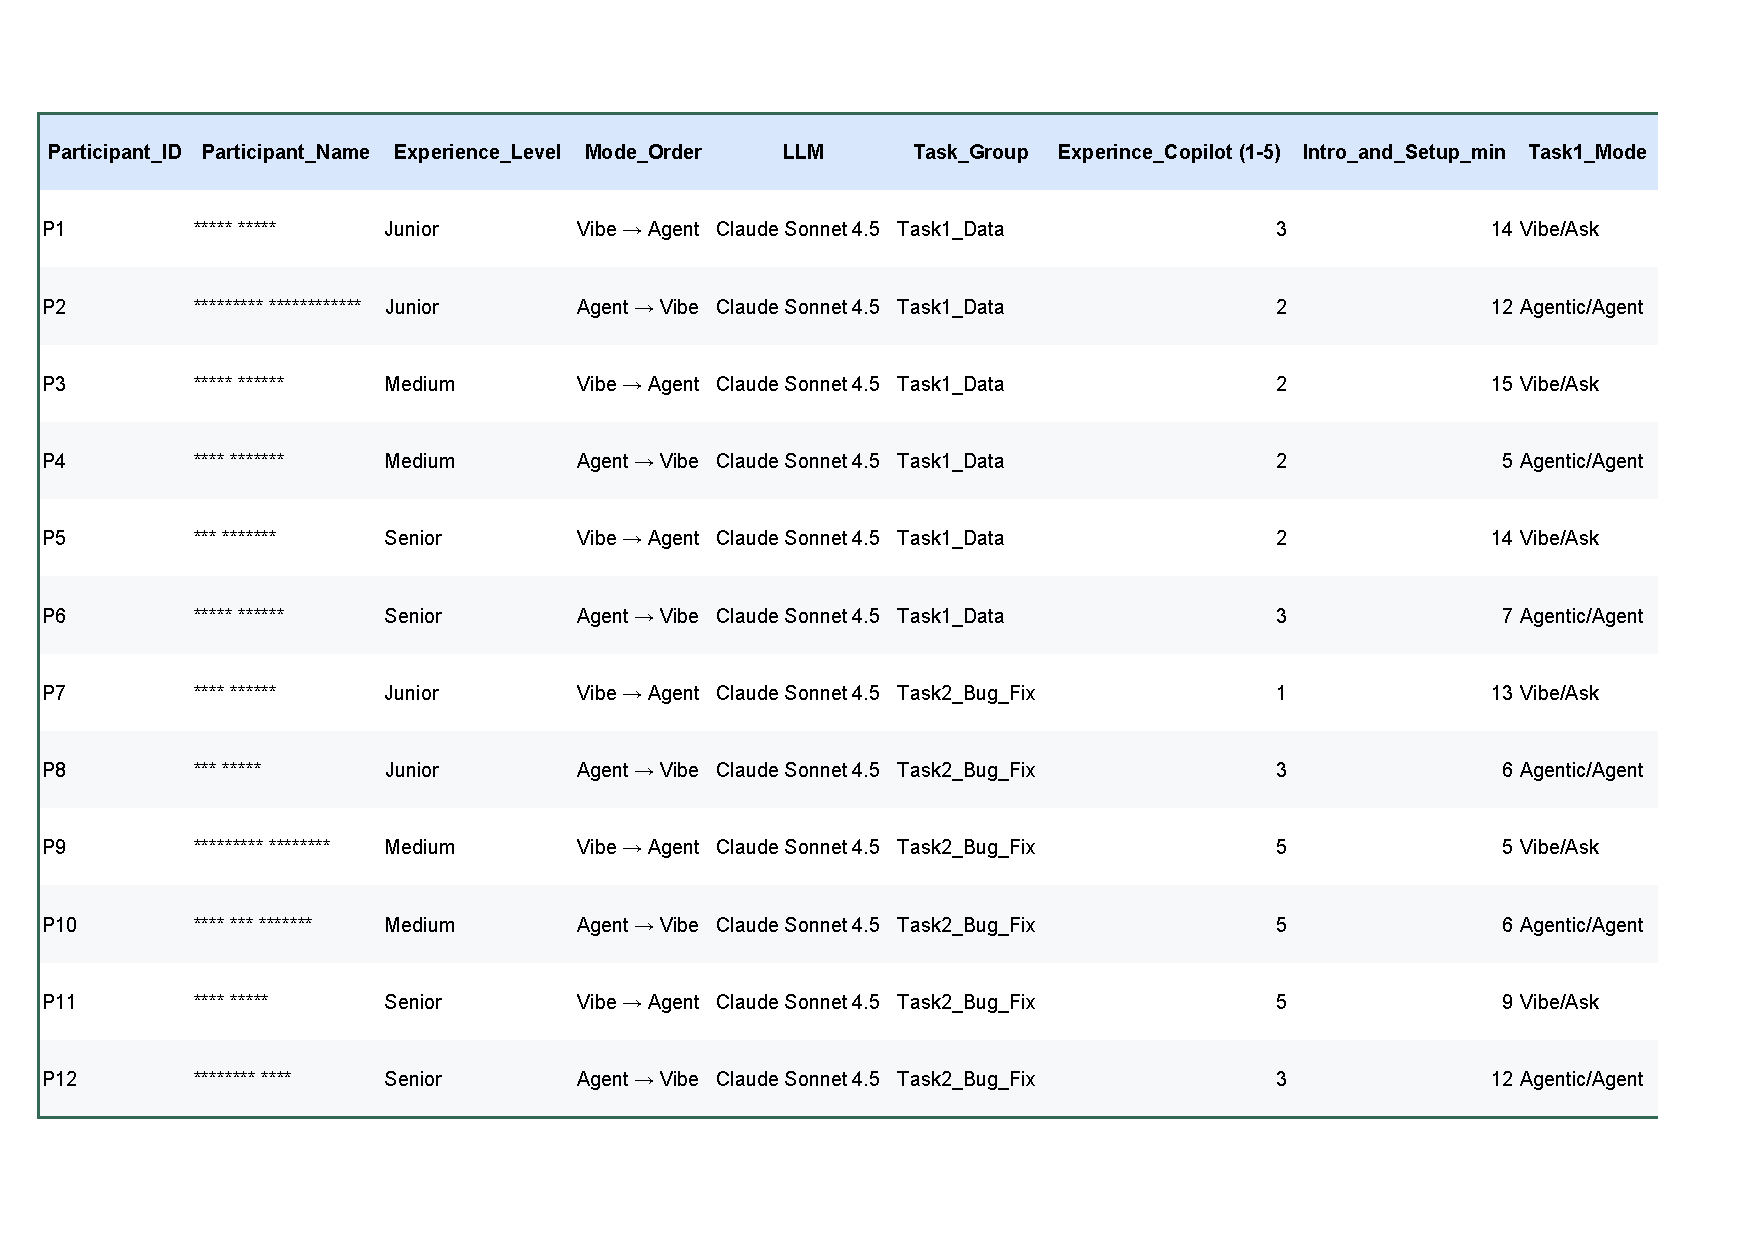
\includepdf[
  pages=-,
  fitpaper=true,
  scale=1,
  offset=0 0,
  pagecommand={\thispagestyle{plain}}
]{figures/master_thesis.pdf}
\end{landscape}



\end{appendices}
